% ============================================================================
% Satellite-Informed Bayesian Storm Modelling for Parametric Flood Risk Pricing
% Proposal to the European Space Agency
%
% LaTeX replication of "ESA Proposal.pages.pdf"
% Compile with: pdflatex esa_proposal.tex   (run twice for references)
% ============================================================================
\documentclass[11pt]{article}

% --- Page geometry -----------------------------------------------------------
\usepackage[a4paper,margin=2.2cm]{geometry}

% --- Fonts: sans-serif body to match the Pages original -----------------------
\usepackage[T1]{fontenc}
\usepackage[utf8]{inputenc}
\usepackage{helvet}
\renewcommand{\familydefault}{\sfdefault}
\usepackage{sansmathfonts} % sans-serif maths so Greek symbols match the body

% --- Layout & typography -----------------------------------------------------
\usepackage{microtype}
\usepackage{parskip}            % block paragraphs (space, no indent) as in original
\usepackage{enumitem}
\setlist[itemize]{leftmargin=1.6em,topsep=4pt,itemsep=4pt}
\setlist[enumerate]{leftmargin=2.0em,topsep=4pt,itemsep=6pt}

% --- Tables ------------------------------------------------------------------
\usepackage{tabularx}
\usepackage{array}
\usepackage{booktabs}
\usepackage{ragged2e}
\renewcommand{\arraystretch}{1.35}
\newcolumntype{L}[1]{>{\RaggedRight\arraybackslash}p{#1}}

% --- Graphics ----------------------------------------------------------------
\usepackage{graphicx}
\usepackage{float}

% --- Section styling (bold, sans, generous spacing) --------------------------
\usepackage{titlesec}
\titleformat{\section}{\Large\bfseries}{}{0pt}{}
\titleformat{\subsection}{\large\bfseries}{}{0pt}{}
\titlespacing*{\section}{0pt}{18pt}{8pt}
\titlespacing*{\subsection}{0pt}{14pt}{6pt}

% --- Hyperlinks --------------------------------------------------------------
\usepackage[hidelinks]{hyperref}

% --- Convenience macros ------------------------------------------------------
\newcommand{\mus}{$\mu$}
\newcommand{\sig}{$\sigma$}
\newcommand{\uu}{$u$}
\newcommand{\xig}{$\xi$}

\begin{document}
\sloppy

% ============================================================================
% TITLE BLOCK
% ============================================================================
\begin{flushleft}
{\fontsize{30}{34}\selectfont\bfseries
Satellite-Informed Bayesian Storm Modelling for Parametric Flood Risk Pricing\par}

\vspace{10pt}
{\LARGE Proposal to the European Space Agency\par}

\vspace{16pt}
\noindent\textbf{Submitted by:} National Physical Laboratory (NPL) / [Lead Applicant
Organisation] \textbf{In partnership with:} MKM Research Labs (MKM)

\vspace{12pt}
\noindent\textbf{Date:} June 2026\\
\textbf{Classification:} Pre-Submission Draft
\end{flushleft}

% ============================================================================
\section{Overview}

This proposal seeks funding and a scientific partnership from the European Space
Agency (ESA) to develop a first-of-its-kind, satellite-driven Bayesian framework
for continuously calibrating the storm-intensity parameters that underpin the
pricing of Physical Risk Swaps (PRS) --- a parametric insurance instrument
modelled by MKM on the credit default swap architecture.

The background to the project is the recent work originating by the NPL, together
with collaboration with the Met Office and the Glocal Association of Risk
Professionals (GARP) who have highlighted the lack of standardisation of climate
risk metrics that are leading to limitation of utility of hazard data provided by
commercial vendors for the banking system that currently can only support basic
disclosure and stress scenarios under the guidance of the ECB and BoE.

MKM has designed the Physical Risk Swap to address the associated model and data
challenges by reverse-engineering Credit Default Swaps, enabling parties to price
the cost of flood-hazard protection for an asset and its issuer. The creation of
hazard events, such as floods, is calibrated using static, loosely historically
derived parameters and a Hybrid Normal-Pareto storm intensity distribution. This
stationarity assumption is a known and material limitation: it means that the PRS
spread and payout trigger do not reflect evolving storm climatology driven by
climate change.

This proposal addresses that limitation through two integrated innovations:

\begin{enumerate}
  \item \textbf{Satellite-Informed Bayesian Parameter Evolution} --- replacing
  static scenario parameters with a Bayesian updating framework in which ESA
  Copernicus satellite observations of real flood events continuously condition
  and evolve the four governing storm intensity parameters, anchored and
  constrained by UK government river gauge data.

  \item \textbf{AI-Governed Parameter Attribution and Portfolio Impact Engine}
  --- an artificial intelligence system that monitors parameter evolution,
  attributes change to its satellite-observable causes, and quantifies the
  downstream impact on every live PRS contract and the aggregate portfolio before
  any update is committed to production.
\end{enumerate}

Together, these innovations make the full ESA Earth Observation archive
financially actionable for the first time, and deliver a governance-grade,
metrologically traceable pricing infrastructure for parametric flood risk
transfer.

% ============================================================================
\section{Problem Statement}

To integrate PRS into banking, MKM has extended the use of parametric insurance
that pays a fixed, pre-agreed sum when a measurable physical event crosses an
agreed-upon threshold --- automatically, without loss adjustment. For flood risk,
the trigger is typically a river-gauge level or a satellite-derived inundation
extent at a specified location. This mechanism eliminates claims disputes and
accelerates capital deployment to affected parties, making parametric instruments
increasingly central to sovereign, infrastructure, and corporate flood risk
management in emerging markets, thereby improving access to capital markets by
stripping out and hedging hazard risk.

The Physical Risk Swap (PRS) extends this architecture using the modelling
conventions of credit default swaps. The PRS calculates:

\begin{itemize}
  \item \textbf{Asset-level pricing:} the cost of protection against flood damage
  to a specific physical asset, modelled from its exposure, vulnerability, and
  local hazard characteristics
  \item \textbf{Gauge-level pricing:} the cost of protection referenced to a
  specific river gauge trigger, modelled from storm intensity distributions and
  the gauge's hydrological response.
  \item \textbf{The basis:} the spread between these two pricing surfaces,
  representing the residual trigger risk --- the possibility that a flood damages
  the asset without breaching the gauge trigger, or vice versa
\end{itemize}

The expectation is that indices constructed from a basket of gauges will evolve
into liquid, tradable assets that will support superior capital allocation and, in
turn, improved credit allocation to climate-related remediation initiatives. Banks
are left to measure the basis risk between the hazard-risk underwriting at the
asset level and the gauges they are expected to use as hedging instruments.

Measuring basis risk is the central commercial and regulatory challenge for
parametric flood insurance. Given that floods occur less frequently at the asset
level than at gauges located on local minima in the catchment area, the
reassessment of the basis naturally occurs infrequently, placing the solution at
risk of tracking short- and medium-term weather patterns.

In a capital markets setting of intra-day trading, the PRS platform needs to
operate under a near-continuous reassessment of the assumptions embedded in the
storm modelling. This feature aligns closely with the strategic desire of the ESA
to act as an early-warning service to enable immediate remediation actions that
save lives and minimise asset damage.

% ============================================================================
\section{The Stationarity Problem}

The PRS platform is currently available as an open-source solution on the
MKM-Research-Labs GitHub site. The PRS pricing engine is fed by the MKM Storm
Intensity Distribution Model (MKM-SI-001), a Hybrid Normal-Pareto probability
distribution governed by four parameters:

\begin{itemize}
  \item \textbf{\mus{} (base mean):} Controls the central tendency of storm
  intensity
  \item \textbf{\sig{} (base standard deviation):} Controls the spread of typical
  events
  \item \textbf{\uu{} (tail threshold):} The intensity level above which extreme
  Pareto scaling engages
  \item \textbf{\xig{} (tail index):} Controls the heaviness of the extreme tail
  --- the single most influential parameter for return-period intensities and
  therefore PRS pricing
\end{itemize}

These parameters are currently calibrated to a historical storm catalogue using
maximum-likelihood estimation (body) and Hill estimation (tail), and then held
constant within each of five predefined scenario families. The model
documentation explicitly flags stationarity as a primary limitation: it does not
account for climate change trends or decadal variability driven by ENSO, NAO, or
AMO oscillations.

The consequence for PRS pricing is outlined in their model risk documentation:

\begin{itemize}
  \item \textbf{Spread under-pricing} when storm climatology is intensifying ---
  the tail index \xig{} is too high (thin tail), under-stating extreme event
  frequency.
  \item \textbf{Trigger mis-calibration} when the threshold \uu{} does not reflect
  the gauge level distribution under current climate conditions.
  \item \textbf{Basis misstatement} when asset-level and gauge-level models
  diverge due to spatially heterogeneous shifts in storm behaviour that a single
  national parameter set cannot capture
\end{itemize}

% ============================================================================
\section{The Data Opportunity}

ESA's Copernicus programme provides a systematic, continuous, globally consistent
archive of satellite observations capable of characterising individual storm
events with sufficient fidelity to inform parameters of the storm intensity
distribution. The Sentinel-1 SAR constellation --- operating since 2014,
cloud-penetrating, and capable of day-and-night operation --- delivers observed
flood extents within hours of inundation onset. The Copernicus Emergency
Management Service (CEMS) Global Flood Monitoring (GFM) service produces
near-real-time flood maps from every Sentinel-1 acquisition, providing a
consistent, near-decade-long flood event catalogue.

Simultaneously, the UK National River Flow Archive (NRFA), operated by the UK
Centre for Ecology and Hydrology, provides freely accessible, quality-controlled
daily mean flow and peak flow data from over 1,600 gauging stations across the
United Kingdom --- precisely the gauge network that underpins PRS trigger
calibration.

The scientific and pre-commercial opportunity is to connect these two data
streams --- satellite-observed flood events and gauge-measured hydrological
responses --- through an AI-mediated Bayesian framework that continuously updates
the PRS pricing parameters to reflect realised storm behaviour.

% ============================================================================
\section{Conceptual Architecture}

The proposed system operates as a closed-loop Bayesian calibration engine
positioned between the ESA data infrastructure and the PRS pricing stack. Its
operation can be described in five stages:

\begin{itemize}
  \item \textbf{Stage 1 --- Event Detection.} Sentinel-1 SAR acquisitions are
  continuously monitored via the Copernicus Data Space Ecosystem (CDSE) API. When
  CEMS GFM produces a new flood extent product, an event is registered. The event
  is characterised by its spatial footprint, inundation area, onset rate, peak
  extent, and duration --- all derivable from the time-sequential SAR archive
  using the Copernicus DEM for terrain context.

  \item \textbf{Stage 2 --- Intensity Scoring.} The observed physical event must be
  placed on the MKM normalised intensity scale (0--100). This requires a
  \textbf{transfer function} that maps multi-dimensional physical observables
  (inundation area in km\textsuperscript{2}, duration in hours, rate of onset,
  spatial coherence across the catchment) to a scalar intensity score. Because the
  satellite observes flood \textit{extent} --- which the MKM chain itself produces
  from gauge levels through its hydrological (Hydrograph, MKM-HG-001) and hydraulic
  (Flood Propagation) models --- the transfer function is effectively an inversion
  of that physical chain. It must be validated for consistency against it. This
  transfer function is the most scientifically challenging component of the system,
  and the primary locus of NPL's metrological contribution. The function must:
  \begin{itemize}
    \item Produce a traceable, uncertainty-quantified intensity score with
    defensible confidence intervals.
    \item Be consistent with the existing MKM model's intensity scale so that
    updates are compatible with the established pricing architecture.
    \item Be anchored by concurrent NRFA gauge observations, which provide an
    independent physical measurement of flood severity at the trigger point.
  \end{itemize}

  \item \textbf{Stage 3 --- Bayesian Parameter Update.} The intensity score,
  together with its uncertainty, is used to update the four governing parameters
  using Bayesian inference. The current parameter set constitutes the prior; the
  observed intensity score provides the likelihood; the posterior becomes the
  updated parameter set for the next pricing cycle. This approach is
  well-established in extreme value hydrology --- hierarchical Bayesian GEV
  frameworks have demonstrated superior flood quantile estimation compared to
  classical methods, particularly for constraining tail behaviour with limited
  data. The update is \textbf{event-triggered}, not time-scheduled: parameters
  evolve in response to observed reality, not the passage of calendar time. Between
  events, the parameters remain stable. This design preserves the governance
  integrity of the Tier 1/2 model chain while ensuring that material new
  information is incorporated promptly.

  \item \textbf{Stage 4 --- Gauge Constraint.} NRFA gauge data serves a dual role.
  First, it acts as a \textbf{likelihood constraint} on the Bayesian update. If the
  satellite-derived intensity score implies a 1-in-50-year event but the gauge
  record indicates a 1-in-10-year event at the relevant station, the update is
  moderated accordingly. Second, it provides a \textbf{direct calibration anchor}
  for the gauge-level PRS pricing surface, ensuring that the asset-level and
  gauge-level models remain coherently coupled. This is the mechanism by which
  basis risk is most directly controlled.

  \item \textbf{Stage 5 --- Impact Attribution and Portfolio Governance.} Before
  any updated parameter set is committed to the live PRS pricing engine, the AI
  attribution system computes the full downstream impact across \textbf{both arms}
  of the model chain. The \textbf{gauge-level (trigger) arm} runs Storm Intensity
  Distribution (MKM-SI-001) $\rightarrow$ Storm-Gauge Response Model (MKM-SG-001)
  $\rightarrow$ GEV Hazard Curve Model (MKM-GH-001) $\rightarrow$ PRS Analytical
  Pricing Model (MKM-PR-001). The \textbf{asset-level (damage) arm} branches at the
  gauge response through the hydrological and hydraulic models --- Hydrograph
  (MKM-HG-001) $\rightarrow$ Flood Propagation $\rightarrow$ Property Flood Response
  (MKM-PF-001) $\rightarrow$ Depth-Damage Curve (MKM-DD-001) --- before recombining
  at the PRS pricing engine. Since the basis is the spread between these two arms,
  attributing each parameter change to its separate effect on each arm is precisely
  what makes the basis impact explicit. For every live PRS contract, the system
  produces a delta report showing the change in spread, trigger probability, and
  expected payout under the proposed updated parameters. The aggregate portfolio
  net present value change is computed and presented to the governance function for
  review. Only upon human approval is the update committed.
\end{itemize}

% ============================================================================
\section{Workstream Structure}

\subsection{Workstream 1 --- Transfer Function Development and Metrological
Calibration}

\textit{Objective:} Construct a validated, traceable transfer function mapping ESA
satellite observables to the MKM intensity scale, constrained by NRFA gauge data.

\textbf{Activities:}
\begin{itemize}
  \item Ingest the Sentinel-1 GRD archive (2014--present) from CDSE for UK flood
  catchments, using the S3 and openEO APIs for cloud-native processing at NPL
  compute infrastructure.
  \item Extract flood event catalogues using CEMS GFM products as the primary
  detection layer, supplemented by independent Sentinel-1 backscatter change
  detection
  \item Characterise each detected event across five physical dimensions: peak
  inundation extent, total inundation volume (derived with Copernicus DEM EEA-10),
  event duration, onset rate, and catchment spatial coherence.
  \item Match each satellite-detected event to concurrent NRFA peak flow and gauge
  level observations at co-located stations, constructing a paired satellite-gauge
  event dataset.
  \item Train and validate the AI transfer function --- mapping the
  five-dimensional physical feature vector to a scalar intensity score with
  calibrated uncertainty --- using NPL standards for uncertainty propagation.
  \item Validate the transfer function against the existing MKM historical scenario
  calibration (\mus{}=40, \sig{}=12, \uu{}=60, \xig{}=3.0) to ensure scale
  consistency.
\end{itemize}

\textit{Key output:} A validated, governance-ready transfer function with traceable
uncertainty bounds, certified by NPL as fit for use in a Tier 2 pricing model.

\subsection{Workstream 2 --- Bayesian Parameter Evolution Engine}

\textit{Objective:} Implement and validate the Bayesian updating framework that
evolves the four MKM parameters in response to observed events.

\textbf{Activities:}
\begin{itemize}
  \item Establish the Bayesian prior from the existing five MKM scenario families,
  treating the historical scenario as the initial prior distribution over
  (\mus{}, \sig{}, \uu{}, \xig{}).
  \item Define the likelihood function for each parameter, informed by the transfer
  function output from WS1 and the NRFA gauge constraint.
  \item Implement the posterior update using Markov Chain Monte Carlo (MCMC)
  sampling, consistent with established Bayesian GEV frameworks for flood frequency
  analysis.
  \item Test the update mechanics against a held-out set of known UK flood events
  (e.g. 2019--20 England floods, 2021 Yorkshire flooding) to verify that the
  Bayesian updates move parameters in physically meaningful directions.
  \item Define and implement governance gates: criteria for classifying an update
  as material (requiring human review) versus immaterial (logged but not
  propagated), informed by the model's existing sensitivity analysis showing that
  \xig{} changes near 1.0 have non-linear, amplified effects.
  \item Produce a new extended scenario family --- a \textbf{Dynamic Climate
  Scenario} --- that represents the current posterior parameter distribution as a
  living, updatable member of the MKM scenario family table.
\end{itemize}

\textit{Key output:} A functioning Bayesian update engine integrated with the MKM
Storm Intensity Distribution Model, with documented governance triggers and a
validated update audit trail.

\subsection{Workstream 3 --- AI Attribution and Portfolio Impact Engine}

\textit{Objective:} Build the AI system that quantifies the downstream PRS
portfolio impact of each proposed parameter update and supports the governance
review workflow.

\textbf{Activities:}
\begin{itemize}
  \item Instrument the full MKM model chain --- the gauge-level arm (MKM-SI-001
  $\rightarrow$ MKM-SG-001 $\rightarrow$ MKM-GH-001 $\rightarrow$ MKM-PR-001) and
  the asset-level arm that branches through the hydrological and hydraulic models
  (MKM-SG-001 $\rightarrow$ Hydrograph MKM-HG-001 $\rightarrow$ Flood Propagation
  $\rightarrow$ Property Flood Response MKM-PF-001 $\rightarrow$ Depth-Damage
  MKM-DD-001 $\rightarrow$ MKM-PR-001) --- to accept parameter perturbations and
  propagate them to PRS contract-level outputs
  \item Develop the attribution engine: for any proposed ($\Delta$\mus{},
  $\Delta$\sig{}, $\Delta$\uu{}, $\Delta$\xig{}), compute the partial derivatives
  of spread, trigger probability, and expected payout with respect to each
  parameter, attributing total impact to its constituent drivers.
  \item Implement the portfolio delta report: for each live PRS contract, report
  the changes in mark-to-market value, spread, trigger exceedance probability, and
  expected payout under the proposed updated parameters.
  \item Build the governance workflow interface: present the attribution report and
  portfolio delta to the approving authority with sufficient context (event
  summary, satellite evidence, gauge data) to support an informed decision; log all
  approvals and rejections for the regulatory audit trail.
  \item Design and implement the model monitoring dashboard: track the evolution of
  (\mus{}, \sig{}, \uu{}, \xig{}) over time, alert when parameters drift beyond
  predefined bands relative to the scenario family ladder, and flag any parameter
  combination that approaches the \xig{} $<$ 1.5 region where the distribution has
  infinite variance
\end{itemize}

\textit{Key output:} A production-grade AI attribution and governance engine,
integrated with the PRS platform, capable of processing parameter updates within
the existing Tier 1/2 model risk governance framework.

% ============================================================================
\section{Data Architecture}

\begin{figure}[H]
  \centering
  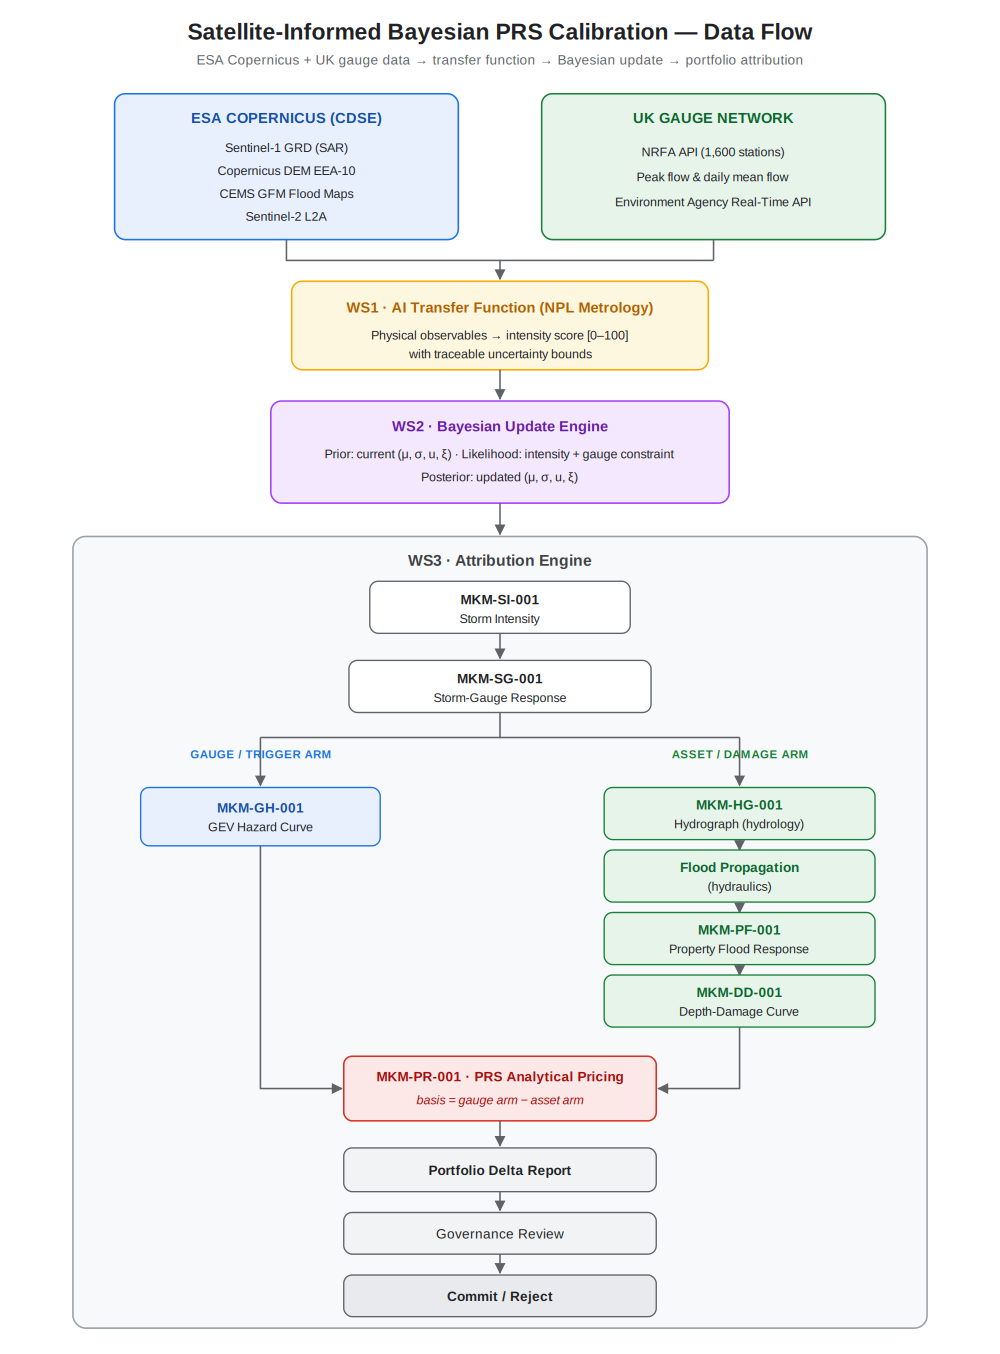
\includegraphics[width=\textwidth,keepaspectratio]{data_flow_diagram.png}
  \caption*{Satellite-Informed Bayesian PRS Calibration --- Data Flow. ESA
  Copernicus + UK gauge data $\rightarrow$ transfer function $\rightarrow$ Bayesian
  update $\rightarrow$ portfolio attribution.}
\end{figure}

\subsection{Primary ESA Data Stack}

\begin{table}[H]
\centering
\begin{tabularx}{\textwidth}{L{3.1cm} L{2.8cm} L{2.0cm} X}
\toprule
\textbf{Data Layer} & \textbf{Source} & \textbf{Access Method} & \textbf{Role}\\
\midrule
Sentinel-1 GRD (COG\_SAFE) & Copernicus Data Space Ecosystem & S3 / openEO API &
Event detection, flood extent characterisation\\
Copernicus DEM EEA-10 (10\,m) & CDSE & S3 & Inundation volume estimation, flow
routing\\
CEMS GFM Products & CEMS Early Warning Data Store & REST API & Primary flood event
catalogue, detection benchmark\\
Sentinel-2 L2A & CDSE & STAC / openEO & Pre-event land cover, optical validation
(clear sky)\\
Copernicus Land Monitoring --- Imperviousness & land.copernicus.eu & WCS & Urban
runoff characterisation for catchment context\\
\bottomrule
\end{tabularx}
\end{table}

All ESA data is available free of charge under the Copernicus open data policy
following registration. The cloud-native CDSE infrastructure, which holds over 78
petabytes of immediately accessible data, enables processing at scale without bulk
data transfer by using the openEO API for server-side computation.

\subsection*{UK Government Gauge Data}

\begin{table}[H]
\centering
\begin{tabularx}{\textwidth}{L{3.1cm} L{2.8cm} L{2.4cm} X}
\toprule
\textbf{Data Layer} & \textbf{Source} & \textbf{Access Method} & \textbf{Role}\\
\midrule
Daily mean flow & NRFA API (CEH) & REST API / CSV & Gauge constraint on Bayesian
update\\
Peak flow dataset & NRFA API (CEH) & REST API / WINFAP & Flood frequency baseline
for prior calibration\\
Near-real-time gauge levels & Environment Agency API & REST API & Live trigger
monitoring for PRS event detection\\
\bottomrule
\end{tabularx}
\end{table}

The NRFA API provides freely accessible daily mean flows, catchment daily rainfall,
and peak flow data from over 1,600 UK gauging stations in JSON or CSV format. This
data is openly licensed under the Open Government Licence.

% ============================================================================
\section{Alignment with ESA Priorities}

This project directly instantiates ESA's Earth Action ambition: translating
satellite data into tangible societal and economic decisions. The PRS is a
financial mechanism for flood risk transfer --- making flood protection
economically accessible and efficiently priced. Better-priced parametric insurance
instruments accelerate capital deployment to flood-affected communities and assets,
reducing the protection gap, one of the most significant economic consequences of
climate change.

This proposal aligns directly with the open Horizon Europe call
HORIZON-CL6-2026-03-GOVERNANCE-01: ``Develop Earth Intelligence solutions using
environmental observations and state-of-the-art AI for sustainable competitiveness
and policy making''. Specifically:

\begin{itemize}
  \item \textbf{Intensive use of Copernicus EO data:} Sentinel-1 SAR, Copernicus
  DEM, and CEMS GFM are the primary data inputs throughout all three workstreams
  \item \textbf{AI-driven decision support tools for private actors:} The PRS
  pricing engine and attribution system directly serve financial institutions,
  insurers, and corporate treasuries managing flood exposure.
  \item \textbf{Co-design with end-users:} The PRS platform operator (project lead)
  is an end-user co-designer, ensuring fit-for-purpose outputs from the first
  workstream
  \item \textbf{Explainability and robustness:} The Bayesian attribution
  architecture provides explicit, auditable explanations for every parameter change
  and its portfolio consequences
  \item \textbf{Collaboration with ESA FutureEO:} The project explicitly builds on
  and extends the CEMS GFM service and the Copernicus Data Space Ecosystem
  infrastructure, with commitment to ESA FutureEO coordination activities
\end{itemize}

The project also aligns with ESA Phi-Lab UK Pillar 1: Fight climate change with
space technology. Parametric flood insurance priced on satellite-derived,
climate-evolving storm parameters is a direct commercial application of space
technology to climate adaptation. Phi-Lab UK offers funding of
\texteuro{}200,000--\texteuro{}225,000 per project for UK-based applicants from
private organisations, research institutions, and academia, with NPL and the
project lead constituting an eligible UK-based consortium.

% ============================================================================
\section{Innovation and Novelty}

This project is novel across three dimensions:

\begin{itemize}
  \item \textbf{Scientific novelty.} While Bayesian GEV frameworks for flood
  frequency analysis are established in hydrology, their application to the
  continuous, event-triggered calibration of a parametric pricing model parameter
  set --- specifically using the Hybrid Normal-Pareto intensity scale of the MKM
  architecture --- has not been demonstrated. The integration of SAR-derived flood
  observables as the likelihood function in such an update represents a genuinely
  new methodological contribution.

  \item \textbf{Commercial novelty.} The use of Earth Observation data as a dynamic
  input to an open source structured financial product's pricing engine --- rather
  than solely as a payout trigger --- is a frontier application of satellite data in
  capital markets. The PRS-based quantification enabled by co-registered satellite
  and gauge observations represents a step change in the precision of parametric
  flood pricing.

  \item \textbf{Governance novelty.} The AI attribution engine --- which quantifies
  the downstream portfolio impact of satellite-informed parameter changes before
  they are committed --- establishes a new standard for model risk governance in
  EO-informed financial applications. The architecture explicitly preserves the
  Tier 1/2 governance hierarchy of the existing MKM model framework, demonstrating
  that satellite-driven dynamism and financial regulatory compliance are not in
  tension.
\end{itemize}

% ============================================================================
\section{Known Limitations and Risk Mitigations}

\begin{table}[H]
\centering
\begin{tabularx}{\textwidth}{X X}
\toprule
\textbf{Limitation} & \textbf{Mitigation}\\
\midrule
Transfer function uncertainty: mapping physical observables to the normalised
[0--100] scale involves irreducible modelling judgement &
NPL metrological framework provides traceable uncertainty bounds; Bayesian update
propagates this uncertainty into parameter posteriors rather than treating the
score as exact\\
Sentinel-1 archive length (from 2014): $\sim$12 years is insufficient to
independently estimate decadal or centennial return periods &
NRFA peak flow archive (from 1960s at many stations) constrains long-return-period
tail behaviour; the Bayesian prior from the existing MKM historical scenario
encodes pre-satellite climatological knowledge\\
Independence assumption in the storm intensity model: temporal clustering of storm
events is not captured in the current MKM architecture &
WS2 Bayesian update operates on individual event observations; cluster sequences
are characterised using the storm sequence parameters documented in test results
(MKM-SS-001)\\
UK-focus of NRFA gauge data: limits immediate applicability to UK PRS portfolios &
Initial scope is explicitly UK; extension to European gauge networks (EuroWQMS,
GRDC) is a future phase deliverable\\
Stationarity of the transfer function itself: the satellite-to-intensity mapping
may itself evolve &
Annual model review of transfer function parameters is included in the project
governance cycle, consistent with existing SR 26/2 requirements for annual review\\
\bottomrule
\end{tabularx}
\end{table}

% ============================================================================
\section{Conclusion}

The convergence of ESA's systematic satellite observation programme, the UK's
world-class river gauge network, and advances in Bayesian inference and AI
attribution creates a unique opportunity to develop a new generation of
climate-responsive parametric flood-pricing instruments. The Physical Risk Swap ---
already a sophisticated financial engineering achievement modelled on credit
default swap architecture --- has a clear and addressable limitation: its governing
storm-intensity parameters do not evolve in response to observed reality.

This proposal provides the scientific framework, the data infrastructure, and the
governance architecture to close that gap. By making the ESA Copernicus archive
financially actionable through metrologically rigorous AI, this project delivers
direct societal impact for ESA by improving flood risk transfer, advances the
scientific state-of-the-art in Bayesian EO-to-parameter calibration, and
establishes a replicable governance model for satellite-informed financial products
that will extend far beyond flood risk. The project is ready to proceed. The model
architecture is in place, the financial modelling and governance infrastructure is
in place, and the partnership between domain expertise (MKM Research Labs),
measurement science (NPL), and satellite data (ESA) is uniquely configured to
deliver this outcome.

The Earth Observation ingestion, the metrologically calibrated transfer function,
the Bayesian parameter-evolution engine, and the AI attribution engine are the
funded deliverables of the workstreams above; the readiness review in Part B sets
out precisely which foundations already exist to build upon.

\end{document}
